\documentclass[9pt,twocolumn,a4paper]{extarticle}

\usepackage{amsmath}
\usepackage{fontspec}
\usepackage{unicode-math}
\setmainfont{CharisSIL-Regular.ttf}[BoldFont=CharisSIL-Bold.ttf,ItalicFont=CharisSIL-Italic.ttf,BoldItalicFont=CharisSIL-BoldItalic.ttf]
\setmathfont{STIXTwoMath-Regular.otf}
\setmonofont{consola.ttf}[BoldFont=consolab.ttf,ItalicFont=consolai.ttf,Scale=0.9]
\usepackage[top=1.5cm,bottom=2.3cm,left=1.35cm,right=1.35cm,columnsep=0.75cm,footskip=0.9cm,headsep=0.45cm]{geometry}
\usepackage{graphicx}
\usepackage{booktabs}
\usepackage{array}
\usepackage{xcolor}
\usepackage{titlesec}
\usepackage{caption}
\usepackage{float}
\usepackage{tikz}
\usetikzlibrary{arrows.meta,positioning}
\usepackage{fancyhdr}
\usepackage{microtype}

\definecolor{linkblue}{RGB}{0,106,150}
\definecolor{bannergray}{RGB}{229,229,229}
\usepackage[colorlinks=true,linkcolor=linkblue,citecolor=linkblue,urlcolor=linkblue]{hyperref}

\tikzset{
  pbox/.style={draw=linkblue,thick,rounded corners=2pt,fill=linkblue!8,align=center,
               minimum height=9mm,text width=19mm,font=\footnotesize},
  pmine/.style={pbox,fill=linkblue!25,very thick},
  parr/.style={-{Stealth[length=2mm]},thick}}

\titleformat{\section}{\normalsize\bfseries}{\thesection.}{0.55em}{}
\titleformat{\subsection}{\small\itshape}{\thesubsection.}{0.55em}{}
\titlespacing*{\section}{0pt}{10pt}{4pt}
\titlespacing*{\subsection}{0pt}{7pt}{3pt}
\setlength{\parskip}{0pt}
\setlength{\parindent}{1.1em}
\setlength{\arraycolsep}{2pt}
\setlength{\abovedisplayskip}{4pt}
\setlength{\belowdisplayskip}{4pt}
\renewcommand{\figurename}{Fig.}
\renewcommand{\tablename}{Table}
\renewcommand{\refname}{References}
\captionsetup{font={footnotesize},labelfont=bf,labelsep=period,justification=justified,singlelinecheck=false,skip=3pt}
\captionsetup[table]{position=top}
\emergencystretch=3em
\setlength{\textfloatsep}{9pt plus 2pt minus 2pt}
\setlength{\floatsep}{7pt plus 2pt minus 2pt}
\setlength{\intextsep}{7pt plus 2pt minus 2pt}
\linespread{1.04}
\raggedbottom

\newcommand{\code}[1]{\texttt{#1}}
\newcommand{\spaced}[1]{\textls[160]{#1}}
% "Intuition" and "In CocCoc Plus" boxes
\newcommand{\idea}[1]{\par\vspace{3pt}\noindent\fcolorbox{linkblue}{linkblue!6}{\parbox{\dimexpr\columnwidth-2\fboxsep-2\fboxrule}{\footnotesize\textbf{Intuition.} #1}}\par\vspace{3pt}}
\newcommand{\inproj}[1]{\par\vspace{3pt}\noindent\fcolorbox{gray!60}{gray!6}{\parbox{\dimexpr\columnwidth-2\fboxsep-2\fboxrule}{\footnotesize\textbf{In CocCoc Plus.} #1}}\par\vspace{3pt}}

\newcommand{\runauthor}{\textit{L.\,A.\ Kiet}}
\newcommand{\runtitle}{\textit{How a search engine works: the core formulas and algorithms}}
\pagestyle{fancy}
\fancyhf{}
\renewcommand{\headrulewidth}{0pt}
\fancyhead[L]{\footnotesize\runauthor}
\fancyhead[R]{\footnotesize\runtitle}
\fancyfoot[C]{\footnotesize\thepage}
\fancypagestyle{first}{\fancyhf{}\renewcommand{\headrulewidth}{0pt}}

\makeatletter
\renewcommand\@biblabel[1]{\textcolor{linkblue}{[#1]}}
\makeatother

\begin{document}
\thispagestyle{first}

\twocolumn[{%
\begin{@twocolumnfalse}
\vspace{-0.3cm}
\begin{center}\small\color{linkblue}Data Structures and Algorithms, course project companion notes (2026)\end{center}
\vspace{-0.1cm}
\noindent\rule{\textwidth}{0.5pt}\\[-2pt]
\noindent\colorbox{bannergray}{\parbox{\dimexpr\textwidth-2\fboxsep}{\centering\vspace{3pt}
  {\small Course: Data Structures and Algorithms \;$\cdot$\; International University, VNU-HCM}\\[7pt]
  {\Large Background notes for CocCoc Plus}\vspace{4pt}}}\\[-1pt]
\noindent\rule{\textwidth}{2.2pt}

\vspace{0.55cm}
{\fontsize{16.5}{20}\selectfont How a search engine works:\\the core formulas and algorithms, explained with small examples\par}
\vspace{0.4cm}
{\large Le Anh Kiet\textsuperscript{\,a}\par}
\vspace{0.2cm}
{\scriptsize\textsuperscript{a}\,\textit{International University, Vietnam National University Ho Chi Minh City, Vietnam} \quad Student ID: ITCSIU24047\par}
\vspace{0.3cm}
\noindent\rule{\textwidth}{0.4pt}
\vspace{0.25cm}

\noindent\begin{minipage}[t]{0.255\textwidth}
{\footnotesize\spaced{K E Y W O R D S}\par}
\vspace{2pt}\noindent\rule{\linewidth}{0.4pt}\par\vspace{3pt}
{\scriptsize
Web crawling, Bloom filter\\
Vietnamese word segmentation\\
Inverted index, VByte\\
Posting list intersection\\
TF-IDF, BM25, PageRank\\
Top-$K$ heap, LRU cache\\
MRR, MAP, nDCG\par}
\end{minipage}\hfill
\begin{minipage}[t]{0.715\textwidth}
{\footnotesize\spaced{A B S T R A C T}\par}
\vspace{2pt}\noindent\rule{\linewidth}{0.4pt}\par\vspace{3pt}
{\scriptsize\setlength{\parindent}{0pt}\linespread{1.08}\selectfont
These notes collect the ideas a reader needs before opening the CocCoc Plus source code or its project report. Every formula comes with a short explanation of what it measures and a worked example small enough to check by hand.

The order follows the path of a page through the system. A crawler downloads pages and uses a Bloom filter to remember which URLs it has seen. A word segmenter turns Vietnamese syllables into words with dynamic programming. An inverted index maps each word to the documents that contain it, stored compactly with delta and VByte coding. The query engine intersects these lists, and the ranker scores the survivors with TF-IDF or BM25, adjusted by PageRank and title match. A heap keeps the best ten results. The last section shows how to measure whether the ranking is any good.

Each section ends with a box giving the parameter values that CocCoc Plus uses, so the notes can also be read as a map of the code.\par}
\end{minipage}

\vspace{0.25cm}
\noindent\rule{\textwidth}{0.4pt}
\vspace{0.35cm}
\end{@twocolumnfalse}
}]

%====================================================================
\section{The four jobs of a search engine}
\label{sec:overview}
%====================================================================
A search engine answers a question like ``which pages talk about \emph{giá vàng hôm nay}?'' in a fraction of a second, over a collection far too large to read at query time. It does this by splitting the work into four jobs \cite{manning2008ir}. Two of them run ahead of time and two run when the user presses Enter (Fig.~\ref{fig:pipeline}).

\begin{figure}[H]
\centering
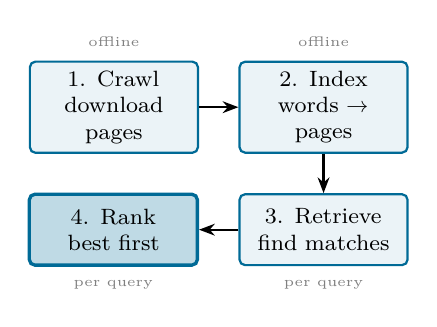
\begin{tikzpicture}[node distance=5mm and 5mm]
  \node[pbox] (crawl) {1. Crawl\\download pages};
  \node[pbox,right=of crawl] (index) {2. Index\\words $\to$ pages};
  \node[pbox,below=of index] (retr) {3. Retrieve\\find matches};
  \node[pmine,left=of retr] (rank) {4. Rank\\best first};
  \draw[parr] (crawl) -- (index);
  \draw[parr] (index) -- (retr);
  \draw[parr] (retr) -- (rank);
  \node[font=\tiny,gray,above=0.5mm of crawl] {offline};
  \node[font=\tiny,gray,above=0.5mm of index] {offline};
  \node[font=\tiny,gray,below=0.5mm of retr] {per query};
  \node[font=\tiny,gray,below=0.5mm of rank] {per query};
\end{tikzpicture}
\caption{The four jobs. Crawling and indexing prepare data in advance, so the two per-query jobs only touch a small part of it.}
\label{fig:pipeline}
\end{figure}

The whole design rests on one trade: spend time and memory offline so that each query is cheap. The index is the result of that trade. Instead of scanning every page for the query words, the engine looks up a precomputed list for each word.

Table~\ref{tab:notation} fixes the symbols used in the rest of the notes.

\begin{table}[H]
\centering
\caption{Notation.}
\label{tab:notation}
\footnotesize
\begin{tabular}{@{}lp{5.6cm}@{}}
\toprule
Symbol & Meaning \\
\midrule
$N$ & number of documents in the collection \\
$t$, $d$, $q$ & a term (word), a document, a query \\
$tf_{t,d}$ & how many times $t$ occurs in $d$ \\
$df_t$ & how many documents contain $t$ \\
$|d|$, $\overline{|d|}$ & length of $d$ in tokens, and the average length \\
$K$ & number of results shown (usually 10) \\
\bottomrule
\end{tabular}
\end{table}

%====================================================================
\section{Crawling the web}
\label{sec:crawl}
%====================================================================
The web is a directed graph: pages are nodes and links are edges. A crawler explores this graph starting from a few seed pages. In its simplest form it is breadth-first search: take a URL from a queue, download the page, extract its links, and put the new ones at the back of the queue. The queue is called the \emph{frontier}.

Three questions turn this textbook BFS into a working crawler. Which URL should be downloaded next? How do we avoid hammering one server? How do we remember millions of visited URLs cheaply?

\subsection{Priority: which page next}
Pages close to the seeds tend to be more useful than pages ten clicks away. A simple priority level is the depth $d$, with small bonuses for signals of importance:
\begin{equation}
\ell=\operatorname{clip}\big(d-[\text{host ends in }\code{.vn}]-[\text{backlinks}\ge5],\ 0,\ 4\big).
\label{eq:level}
\end{equation}
Here $[\cdot]$ is 1 when the condition holds and 0 otherwise, and level 0 is the most urgent. If the crawler always served level 0 first, deep pages would starve. It therefore picks a level at random, with weight
\begin{equation}
w_i=2^{\,L-1-i}\qquad(i=0,\dots,L-1).
\label{eq:weight}
\end{equation}
With $L=5$ levels the weights are $16,8,4,2,1$: level 0 is chosen 16 times as often as level 4, and level 4 still gets a turn.

\subsection{Politeness: one request per host per second}
A crawler with 32 threads could send 32 requests to the same news site at once. To prevent that, each host gets a ``ready at'' timestamp, and after every download the timestamp moves one second into the future. The crawler needs the host whose timestamp is smallest, again and again. That is exactly what a \emph{min-heap} gives: the smallest key in $O(1)$, and removal or insertion in $O(\log n)$.

\idea{A heap is a binary tree stored in an array where every parent is smaller than its children. Only the root is guaranteed to be the minimum, which is all a scheduler needs, and keeping that one guarantee is much cheaper than keeping the whole array sorted.}

\inproj{The frontier has 5 priority queues in front and 128 per-host queues behind, following the Mercator design \cite{heydon1999mercator}. The politeness delay is 1000~ms.}

\subsection{Bloom filter: ``have I seen this URL?''}
News sites link to each other heavily, so the same URL turns up many times. Storing every seen URL in a hash set costs hundreds of megabytes on a large crawl. A Bloom filter \cite{bloom1970} answers the same question with a bit array of $m$ bits and $k$ hash functions.

To add a URL $x$, set the $k$ bits $g_0(x),\dots,g_{k-1}(x)$ to 1. To test $x$, check those $k$ bits. If any of them is 0, $x$ was certainly never added. If all are 1, $x$ was \emph{probably} added: other URLs might have set those bits by chance.

After inserting $n$ items, the chance that a new item looks present (a \emph{false positive}) is about
\begin{equation}
p\approx\big(1-e^{-kn/m}\big)^{k}.
\label{eq:bloomfp}
\end{equation}
Turning this around gives the best size and number of hashes for a target $p$:
\begin{equation}
m=\Big\lceil-\frac{n\ln p}{(\ln 2)^2}\Big\rceil,\qquad k=\operatorname{round}\Big(\frac{m}{n}\ln 2\Big).
\label{eq:bloom}
\end{equation}

\textbf{Example.} For $n=200{,}000$ URLs and $p=1\%$: $m=1{,}917{,}012$ bits, about 234~KB, and $k=7$. Plugging back into \eqref{eq:bloomfp} gives $p\approx1.004\%$. The same URLs in a hash set would take tens of megabytes.

Computing seven independent hashes is wasteful. Two base hashes $h_1,h_2$ are enough \cite{kirsch2006}:
\begin{equation}
g_i(x)=\big(h_1(x)+i\,h_2(x)\big)\bmod m.
\label{eq:dhash}
\end{equation}

\idea{A false positive here means the crawler skips a page it never visited. A Bloom filter can never make the opposite mistake, so it never downloads a page twice because of the filter.}

Two copies of an article often live under different URLs (print version, AMP version, tracking parameters). The URL filter cannot see that, so the crawler also hashes the page body with SHA-256 and drops bodies it has seen before.

\inproj{\code{BloomFilter} uses FNV-1a for $h_1$. Each URL passes seven filters, cheapest first: URL rules, Bloom filter, \code{robots.txt}, private-address check (against SSRF), download, language, body hash.}

%====================================================================
\section{Turning text into terms}
\label{sec:text}
%====================================================================
The index stores \emph{terms}, so every page and every query must be cut into terms in exactly the same way. If the page says \code{máy\_tính} and the query becomes \code{máy} + \code{tính}, they will never match.

\subsection{Normalisation}
Before splitting, text is lowercased and Unicode is normalised so that the same letter with a combining accent and the same letter precomposed look identical. For autocomplete it also helps to strip diacritics, so that a user typing ``ha noi'' still finds ``hà nội''.

\subsection{Why Vietnamese needs segmentation}
In English a space separates words. In Vietnamese a space separates \emph{syllables}, and a word can have one to four of them. ``Nhà hàng xóm'' (the neighbour's house) is \code{nhà} + \code{hàng\_xóm}. A greedy method that always takes the longest dictionary word at the current position reads \code{nhà\_hàng} (restaurant) first and is left with \code{xóm}. It cannot undo that choice.

\subsection{Segmentation as a shortest-path problem}
Give each dictionary word a score $w$. A word that is frequent and long should score high. One workable formula, from the \code{coccoc-tokenizer} data \cite{coccoctokenizer}, uses the word frequency $f$ and its number of syllables $L$:
\begin{equation}
w(f,L)=\big(\log_2(f+3)\big)^{a_L}\cdot L^{\,b_L},
\label{eq:wordweight}
\end{equation}
with constants $a_L,b_L$ fitted for each length. The logarithm stops a word that appears two billion times from swamping everything else.

Now place a node between every pair of syllables, numbered $0$ to $n$. Each dictionary word covering syllables $i$ to $j-1$ becomes an edge $i\to j$ with weight $w$. A segmentation is a path from $0$ to $n$, and we want the path with the largest total weight. Let $\text{best}[j]$ be the best total for the first $j$ syllables:
\begin{equation}
\text{best}[0]=0,\quad
\text{best}[j]=\max_{\,j-4\le i<j}\big(\text{best}[i]+w(s_i\dots s_{j-1})\big).
\label{eq:dp}
\end{equation}
All edges point forward, so one left-to-right pass fills the table. Words have at most four syllables, so each step looks back at most four places and the whole sentence costs $O(n)$.

\begin{figure}[H]
\centering
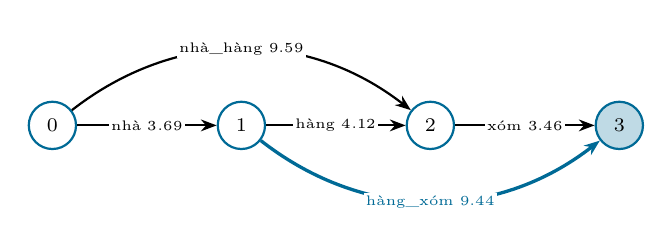
\begin{tikzpicture}[font=\scriptsize,
  nd/.style={circle,draw=linkblue,thick,inner sep=1pt,minimum size=6mm},
  lv/.style={font=\tiny,midway,fill=white,inner sep=0.8pt}]
\node[nd] (n0) at (0,0) {0};
\node[nd] (n1) at (2.4,0) {1};
\node[nd] (n2) at (4.8,0) {2};
\node[nd,fill=linkblue!25] (n3) at (7.2,0) {3};
\draw[parr] (n0)--node[lv]{nhà $3.69$} (n1);
\draw[parr] (n1)--node[lv]{hàng $4.12$} (n2);
\draw[parr] (n2)--node[lv]{xóm $3.46$} (n3);
\draw[parr] (n0) to[bend left=38] node[lv]{nhà\_hàng $9.59$} (n2);
\draw[parr,very thick,linkblue] (n1) to[bend right=38] node[lv]{hàng\_xóm $9.44$} (n3);
\end{tikzpicture}
\caption{Segmentation graph for ``nhà hàng xóm''. The best path $0\to1\to3$ scores $3.69+9.44=13.13$, beating the greedy path $9.59+3.46=13.05$.}
\label{fig:dag}
\end{figure}

\textbf{Example.} For Fig.~\ref{fig:dag}: $\text{best}[1]=3.69$, $\text{best}[2]=\max(3.69+4.12,\ 0+9.59)=9.59$, and $\text{best}[3]=\max(9.59+3.46,\ 3.69+9.44)=13.13$. Following the winning choices backwards gives the cut points $0,1,3$, that is \code{nhà} and \code{hàng\_xóm}.

Names and loanwords are not in the dictionary. Adding a fallback edge of weight $0.5$ from every node to the next one guarantees a path always exists, and because $0.5$ is below every real word, the fallback is only used when nothing else fits.

\inproj{The dictionary sits in a \code{SyllableTrie}: each edge is a whole syllable. If a node has no edge for the next syllable, no word continues that way and the search stops early. Queries and documents go through the same segmenter class.}

%====================================================================
\section{The inverted index}
\label{sec:index}
%====================================================================
A book index lists, for each topic, the pages where it appears. An inverted index does the same for terms: it maps each term to a \emph{posting list}, the sorted list of IDs of documents that contain it. Each posting can also store the positions of the term inside the document, which phrase queries need. The number of positions equals $tf_{t,d}$, so term frequency comes for free.

\begin{figure}[H]
\centering
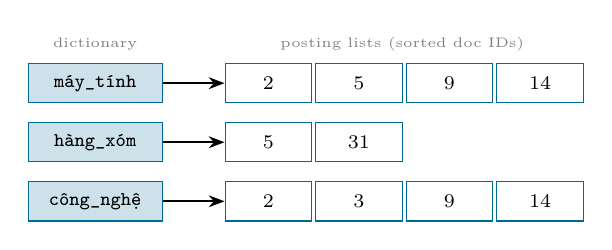
\begin{tikzpicture}[font=\scriptsize,
  cell/.style={draw=linkblue,minimum height=5mm,minimum width=11mm,inner sep=1pt},
  term/.style={cell,fill=linkblue!20,minimum width=17mm}]
\node[term] (t1) at (0,0) {\code{máy\_tính}};
\node[term] (t2) at (0,-0.75) {\code{hàng\_xóm}};
\node[term] (t3) at (0,-1.5) {\code{công\_nghệ}};
\foreach \i/\d in {0/2,1/5,2/9,3/14}
  \node[cell] (a\i) at (2.2+\i*1.15,0) {\d};
\foreach \i/\d in {0/5,1/31}
  \node[cell] (b\i) at (2.2+\i*1.15,-0.75) {\d};
\foreach \i/\d in {0/2,1/3,2/9,3/14}
  \node[cell] (c\i) at (2.2+\i*1.15,-1.5) {\d};
\draw[parr] (t1)--(a0); \draw[parr] (t2)--(b0); \draw[parr] (t3)--(c0);
\node[font=\tiny,gray] at (0,0.5) {dictionary};
\node[font=\tiny,gray] at (3.9,0.5) {posting lists (sorted doc IDs)};
\end{tikzpicture}
\caption{An inverted index. Each term points to the sorted IDs of the documents that contain it.}
\label{fig:inverted}
\end{figure}

Keeping the lists sorted is what makes the rest work: it allows compression by differences, binary search inside a list, and intersection in linear time.

\subsection{Why the lists can be compressed}
Word frequencies follow Zipf's law: the $r$-th most common word appears roughly in proportion to $1/r$ \cite{manning2008ir}. A few terms appear in almost every document and have very long lists. Long lists of sorted IDs have small gaps between neighbours, and small numbers can be written in fewer bytes.

\subsection{Delta coding}
Store the first ID, then the gap to each next one. The list $1002,\,1005,\,1009$ becomes $1002,\,3,\,4$. The original is recovered by a running sum.

\subsection{Variable-byte (VByte) coding}
A plain \code{int} always takes 4 bytes. VByte writes 7 bits of the number per byte, lowest bits first. The top bit of each byte says whether more bytes follow (1) or this is the last one (0). A number $x$ written as bytes with payloads $b_0,b_1,\dots$ is
\begin{equation}
x=\sum_{i} b_i\cdot 128^{\,i}.
\label{eq:vbytesum}
\end{equation}

\textbf{Example.} $300=2\cdot128+44$. The low payload is $44=0101100_2$; more follows, so the first byte is $1\,0101100_2=\code{0xAC}$. The high payload is $2$, the last one, so the second byte is $0\,0000010_2=\code{0x02}$. Two bytes instead of four. Any gap below 128 takes a single byte.

\idea{Delta coding makes the numbers small, and VByte makes small numbers short. Neither step helps much alone.}

Each term's list is compressed separately, so a query only decompresses the few lists it touches. Compressing the whole index file with GZIP would squeeze a little more, but then reading one term would mean unpacking everything.

\inproj{On a 5,011-document corpus with 1,594,938 postings, the lists shrink from 28.1~MB as raw integers to 7.0~MB, i.e.\ to 25\%. A \code{TermDictionary} keeps a single copy of each term string (the Flyweight pattern \cite{gamma1994design}).}

%====================================================================
\section{Finding the matching documents}
\label{sec:query}
%====================================================================

\subsection{Boolean queries}
The simplest model treats a query as a set expression. \code{a b} means ``documents containing both'' (AND, intersection), \code{a OR b} is the union, and \code{-a} removes documents containing \code{a}. A parser turns the text into a tree where each node computes its own set of document IDs. A lone \code{NOT} is never evaluated by itself, since the complement of one list is almost the whole collection. The engine computes the positive part first, then subtracts.

\subsection{Intersecting two sorted lists}
Walk both lists with one pointer each. If the two IDs are equal, output it and advance both. Otherwise advance the pointer at the smaller ID. Each step moves at least one pointer, so the cost is $O(m+n)$.

\textbf{Example.} $A=[2,5,9,14]$ and $B=[3,5,14,20]$. Compare $2<3$, advance $A$; $5>3$, advance $B$; $5=5$, output 5; $9<14$, advance $A$; $14=14$, output 14; $A$ is done. Result: $[5,14]$.

\subsection{Skipping ahead when one list is short}
If $A$ has 10 IDs and $B$ has a million, the two-pointer walk spends almost all its time stepping through $B$. A \code{skipTo}$(t)$ operation jumps to the first ID $\ge t$ in two phases. First it jumps $1,2,4,8,\dots$ positions until it passes $t$ (galloping search). Then it binary-searches inside the last jump. If the target is $\Delta$ positions ahead, this costs $O(\log\Delta)$ instead of $O(\Delta)$.

For queries with several terms, sort the lists by length and intersect from shortest to longest. The running result can only shrink, so later steps are cheap, and the loop stops as soon as the result is empty.

\subsection{Phrase queries}
For \code{"điện thoại giá rẻ"} the engine first intersects the lists of the two terms, then checks positions inside each candidate. The phrase matches if there is a position $p$ of the first term such that term $i$ of the phrase appears at position $p+i$. Positions are sorted, so each check is a binary search.

\inproj{When a long query matches nothing under AND, \code{CandidateResolver} falls back to AND over subsets of its terms, so the user still gets results. The candidate set is capped before ranking.}

%====================================================================
\section{Ranking: which match is best}
\label{sec:rank}
%====================================================================
Retrieval produces a set; the user wants an ordered list. A ranking function gives each candidate a number, and the list is sorted by that number. Good ranking functions agree with three common-sense rules: a document that repeats a query word is more likely to be about it; rare words are more telling than common ones; and a long document mentions many words by chance.

\subsection{TF-IDF and the vector space model}
Treat each document and the query as vectors with one coordinate per term \cite{salton1988}. The weight of term $t$ in document $d$ multiplies two factors:
\begin{equation}
w_{t,d}=\underbrace{\big(1+\log_{10}tf_{t,d}\big)}_{\text{term frequency}}\cdot\underbrace{\log_{10}\frac{N}{df_t}}_{\text{inverse doc. frequency}}.
\label{eq:tfidf}
\end{equation}
The first factor grows slowly: $tf=1,2,10,50$ gives $1,\ 1.30,\ 2,\ 2.70$. The second factor rewards rare terms. With $N=1000$, a term in 10 documents gets $\log_{10}100=2$, while a term in every document gets $\log_{10}1=0$ and stops counting at all.

Two vectors point the same way when their angle is small, so the score is the cosine of that angle:
\begin{equation}
\text{score}(q,d)=\frac{\sum_{t\in q}w_{t,q}\,w_{t,d}}{\lVert q\rVert\cdot\lVert d\rVert}.
\label{eq:cosine}
\end{equation}
The denominator removes the advantage long documents would otherwise have.

\inproj{The sum only runs over query terms. Computing $\lVert d\rVert$ exactly would need every term of $d$, so the code uses $\sqrt{|d|}$ as an approximation.}

\subsection{BM25}
BM25 \cite{robertson2009bm25} comes from a probabilistic model and fixes two weak spots of TF-IDF. Term frequency saturates at a ceiling, and document length is compared with the average:
\begin{equation}
\text{score}(q,d)=\sum_{t\in q}\text{idf}_t\cdot
\frac{tf_{t,d}\,(k_1+1)}{tf_{t,d}+k_1\Big(1-b+b\,\frac{|d|}{\overline{|d|}}\Big)},
\label{eq:bm25}
\end{equation}
\begin{equation}
\text{idf}_t=\ln\Big(1+\frac{N-df_t+0.5}{df_t+0.5}\Big).
\label{eq:bm25idf}
\end{equation}
The two knobs are easy to read. $k_1$ sets how fast repetition stops paying: as $tf$ grows, the fraction approaches $k_1+1$ and never exceeds it. $b$ sets how much length matters: $b=0$ ignores length, $b=1$ divides fully by relative length.

\begin{table}[H]
\centering
\caption{The BM25 term-frequency factor with $k_1=1.2$, $b=0.75$ and average length 200. Repetition saturates, and the same $tf$ counts less in a longer document.}
\label{tab:bm25}
\footnotesize
\begin{tabular}{@{}rrrr@{}}
\toprule
$tf$ & $|d|=100$ & $|d|=200$ & $|d|=400$ \\
\midrule
1 & 1.26 & 1.00 & 0.71 \\
3 & 1.76 & 1.57 & 1.29 \\
10 & 2.05 & 1.96 & 1.82 \\
50 & 2.17 & 2.15 & 2.11 \\
\bottomrule
\end{tabular}
\end{table}

\textbf{Example.} $N=1000$, $df_t=10$: $\text{idf}_t=\ln(1+990.5/10.5)=4.56$. A document of average length with $tf=3$ scores $4.56\times1.57=7.16$ for this term. Going from 10 to 50 repetitions adds only about 10\% (Table~\ref{tab:bm25}), so stuffing a page with keywords gains little.

\inproj{$k_1=1.2$, $b=0.75$, the usual defaults. TF-IDF and BM25 implement the same \code{RelevanceScorer} interface (the Strategy pattern), and \code{APP\_RANKING\_SCORER} picks one at start-up. The idf values are computed once per query, not once per document.}

\subsection{PageRank: importance from links}
Words say whether a page is \emph{about} the query. Links say whether other pages trust it. PageRank \cite{brin1998} imagines a random surfer who, at each step, follows a random link on the current page with probability $\delta$, or jumps to a random page with probability $1-\delta$. The PageRank of a page is the long-run fraction of time the surfer spends there:
\begin{equation}
PR(j)=\frac{1-\delta}{n}+\delta\Big(\sum_{i\to j}\frac{PR(i)}{\text{out}(i)}+\frac{1}{n}\sum_{i\in D}PR(i)\Big).
\label{eq:pagerank}
\end{equation}
Here $n$ is the number of pages, $\text{out}(i)$ the number of links leaving $i$, and $D$ the set of pages with no outgoing links. Their score is spread over all pages; otherwise it would leak away each round. The values always sum to 1.

The equation refers to itself, so it is solved by \emph{power iteration}: start with $PR=1/n$ everywhere, apply \eqref{eq:pagerank} to get new values, and repeat until the change is tiny.

\begin{figure}[H]
\centering
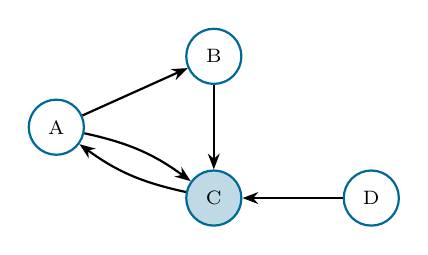
\begin{tikzpicture}[font=\scriptsize,
  nd/.style={circle,draw=linkblue,thick,minimum size=7mm,inner sep=0pt}]
\node[nd] (A) at (0,0) {A};
\node[nd] (B) at (2,0.9) {B};
\node[nd,fill=linkblue!25] (C) at (2,-0.9) {C};
\node[nd] (D) at (4,-0.9) {D};
\draw[parr] (A)--(B);
\draw[parr] (A) to[bend left=12] (C);
\draw[parr] (B)--(C);
\draw[parr] (C) to[bend left=12] (A);
\draw[parr] (D)--(C);
\end{tikzpicture}
\caption{A four-page web. C receives three links, D receives none.}
\label{fig:prgraph}
\end{figure}

\textbf{Example.} For Fig.~\ref{fig:prgraph} with $\delta=0.85$, start from $0.25$ each. After one round, C has $0.0375+0.85(0.25/2+0.25+0.25)=0.569$, since A gives it half its score and B and D give all of theirs. After 28 rounds the values settle at
\[
PR(A)=0.373,\ PR(B)=0.196,\ PR(C)=0.394,\ PR(D)=0.038.
\]
D gets only the random-jump share $0.15/4$. A ranks almost as high as C with a single incoming link, because that link comes from C, the most important page.

\idea{Each round multiplies a link matrix by the vector of scores. The web graph is sparse (most pages link to a tiny fraction of others), so storing only the non-zero entries makes each round cost $O(n+\text{nnz})$, where nnz is the number of links.}

\inproj{$\delta=0.85$, stop when the total change is below $10^{-6}$ or after 100 rounds. On 5,011 pages a dense matrix would need about 191.5~MB; there are only 239,691 links, stored in CSR form (three flat arrays) by \code{SparseMatrix}.}

\subsection{Combining signals}
The final score mixes relevance $s$ (TF-IDF or BM25), PageRank and title match. Adding them with weights, $0.6s+0.3PR$, looks natural but fails when the scales differ. In CocCoc Plus the average TF-IDF score was $0.178$ and the average PageRank $0.00035$, so PageRank contributed about $0.1\%$ of the final score whatever its nominal weight. A safer way multiplies the base score by a boost factor:
\begin{equation}
s'=s\cdot\big(1+\beta\,\widehat{PR}\big),\qquad
\widehat{PR}=\frac{\ln(1+PR/PR_{\min})}{\ln(1+PR_{\max}/PR_{\min})}.
\label{eq:prboost}
\end{equation}
The logarithm squeezes PageRank, which spans several orders of magnitude, into $[0,1]$. For the title, let $\rho\in[0,1]$ be the fraction of query syllables found in the title:
\begin{equation}
s''=s'\cdot(1+\gamma\,\rho).
\label{eq:titleboost}
\end{equation}
Multiplying has two useful properties. The boost does not depend on the scale of $s$, so switching from TF-IDF (scores near $0.18$) to BM25 (near 12) needs no retuning. And a document with $s=0$ stays at 0: authority cannot rescue a page that does not match.

\inproj{$\beta=0.3$, $\gamma=0.1$. Each boost wraps a \code{RelevanceScorer} (the Decorator pattern), so each signal can be switched off to measure its effect.}

%====================================================================
\section{Returning the top ten fast}
\label{sec:topk}
%====================================================================

\subsection{Top-$K$ with a min-heap}
Sorting 30,000 candidates to show 10 wastes work. Keep a min-heap of size $K$ holding the best $K$ seen so far; its root is the weakest of them. For each new candidate, if its score beats the root, replace the root and restore the heap. The cost is $O(n\log K)$ time and $O(K)$ memory, against $O(n\log n)$ for a full sort. With $n=30{,}000$ and $K=10$ that is roughly $30{,}000\cdot\log_2 10\approx 1.0\times10^5$ comparisons, against $4.5\times10^5$. The heap of the first $K$ items can be built in $O(K)$ with \code{heapify}.

\subsection{LRU cache}
Popular queries repeat. A Least-Recently-Used cache keeps the answers to the last $C$ queries and throws away the oldest when full. It combines a hash map (find a key in $O(1)$) with a doubly linked list (move a node to the front or drop the tail in $O(1)$). Every \code{get} moves the entry to the front, so the tail is always the entry unused for the longest time.

\inproj{The search cache holds 200 queries and is rebuilt whenever the index changes. The crawler reuses the same class with capacity 1,000 for DNS lookups.}

\subsection{Autocomplete with a trie}
A trie stores strings character by character, so all strings with a common prefix share a path. To suggest completions for ``hà n'', walk the prefix to its node, collect every suggestion in the subtree, and keep the $K$ most frequent with the same heap trick. Walking a prefix of length $L$ costs $O(L)$ no matter how many strings are stored. Inserting each suggestion twice, once with diacritics and once without, lets ``ha n'' find the same entries.

%====================================================================
\section{Measuring ranking quality}
\label{sec:eval}
%====================================================================
A change to the ranker is only an improvement if a measurement says so. Every metric below needs \emph{relevance judgements}: for each test query, which documents are correct answers.

\subsection{Precision and recall}
If the engine returns a set $R$ and the relevant set is $G$,
\begin{equation}
P=\frac{|R\cap G|}{|R|},\qquad \text{Rec}=\frac{|R\cap G|}{|G|}.
\label{eq:pr}
\end{equation}
Precision asks how much of what we showed is right; recall asks how much of what is right we showed. $P@10$ is precision over the first ten results only, which is what a user actually sees.

\subsection{Rank-aware metrics}
Precision ignores order inside the list. Three metrics fix that.

\textbf{MRR.} If the first correct answer for query $i$ sits at rank $r_i$, the reciprocal rank is $1/r_i$, and
\begin{equation}
\text{MRR}=\frac{1}{|Q|}\sum_{i=1}^{|Q|}\frac{1}{r_i}.
\label{eq:mrr}
\end{equation}
A correct answer at rank 1 gives 1, at rank 2 gives $0.5$, at rank 4 gives $0.25$. Success@1 is the fraction of queries with the answer at rank 1.

\textbf{MAP.} Average precision takes $P@k$ at every rank $k$ where a relevant document appears and averages those values over the relevant documents; MAP averages that over queries.

\textbf{nDCG.} When relevance has grades (0 to 3, say), a highly relevant page at rank 1 should count more than a marginal one. With grade $g_i$ at rank $i$,
\begin{equation}
\text{DCG}@k=\sum_{i=1}^{k}\frac{2^{g_i}-1}{\log_2(i+1)},\qquad
\text{nDCG}@k=\frac{\text{DCG}@k}{\text{IDCG}@k},
\label{eq:ndcg}
\end{equation}
where IDCG is the DCG of the perfect ordering \cite{jarvelin2002}. The logarithm discounts lower ranks, and the division puts the score in $[0,1]$.

\textbf{Example.} Grades in result order $3,2,0,1$ give $\text{DCG}=7+3/1.585+0+1/2.322=9.32$. The ideal order $3,2,1,0$ gives $9.39$, so $\text{nDCG}@4=0.993$. Swapping the last two results costs very little because both sit near the bottom.

\subsection{Is the difference real?}
Two rankers evaluated on 200 queries will rarely tie exactly. To decide whether a gap is more than luck, compare them query by query. A paired $t$-test assumes the per-query differences are roughly normal. A randomisation (permutation) test makes no such assumption: it randomly swaps the two systems' scores on each query many times and counts how often the shuffled gap is as large as the real one \cite{smucker2007}. Reciprocal ranks only take the values $1,\tfrac12,\tfrac13,\dots$, so the permutation test is the safer of the two.

\inproj{The evaluation generates \emph{known-item} queries: pick a document, use its three most distinctive terms (high $tf\cdot idf$, in at least 3 documents and at most 10\% of the corpus) as the query, and treat that document as the only right answer. On 200 such queries, BM25 reaches MRR $0.8989$ (Success@1 $85.0\%$) against $0.8537$ ($78.0\%$) for TF-IDF. Title match lifts TF-IDF to $0.9083$, PageRank only to $0.8625$. A gap counts as significant only if both tests give $p<0.05$ with 100,000 permutations. A further set of 30 hand-written queries with human labels is scored with precision, recall, MAP and nDCG.}

%====================================================================
\section{Cheat sheet}
\label{sec:cheat}
%====================================================================
Table~\ref{tab:complexity} lists the cost of each building block. Most of them trade a small loss (a 1\% false-positive rate, an approximate norm, a heap that only knows its minimum) for a large saving in time or memory.

\begin{table}[H]
\centering
\caption{Cost of the main operations.}
\label{tab:complexity}
\footnotesize
\begin{tabular}{@{}p{2.6cm}p{2.9cm}l@{}}
\toprule
Structure & Operation & Cost \\
\midrule
Min-heap & insert, pop min & $O(\log n)$ \\
 & build from $n$ items & $O(n)$ \\
 & top-$K$ of $n$ & $O(n\log K)$ \\
LRU cache & get, put & $O(1)$ \\
Trie & insert / walk length $L$ & $O(L)$ \\
Bloom filter & add, test & $O(k)$ \\
Segmentation DP & sentence of $n$ syllables & $O(n)$ \\
List intersection & two pointers & $O(m+n)$ \\
 & \code{skipTo} by $\Delta$ & $O(\log\Delta)$ \\
VByte & encode/decode one number & $O(\text{bytes})$ \\
PageRank & one iteration & $O(n+\text{nnz})$ \\
\bottomrule
\end{tabular}
\end{table}

\begin{table}[H]
\centering
\caption{Formulas at a glance.}
\label{tab:formulas}
\footnotesize
\begin{tabular}{@{}p{2.0cm}p{5.6cm}@{}}
\toprule
Topic & Formula \\
\midrule
Bloom size & $m=-n\ln p/(\ln2)^2$, \ $k=(m/n)\ln2$ \\
Segmentation & $\text{best}[j]=\max_i(\text{best}[i]+w(s_i..s_{j-1}))$ \\
VByte & $x=\sum_i b_i\,128^i$ \\
TF-IDF & $(1+\log tf)\cdot\log(N/df)$ \\
BM25 & $\text{idf}\cdot tf(k_1{+}1)/(tf+k_1(1-b+b|d|/\overline{|d|}))$ \\
PageRank & $(1-\delta)/n+\delta\sum_{i\to j}PR(i)/\text{out}(i)$ \\
Boost & $s\,(1+\beta\widehat{PR})(1+\gamma\rho)$ \\
MRR & mean of $1/r_i$ \\
nDCG & $\sum(2^{g_i}-1)/\log_2(i+1)$, divided by ideal \\
\bottomrule
\end{tabular}
\end{table}

\begin{thebibliography}{99}\footnotesize\itemsep0pt\parskip0pt
\bibitem{manning2008ir} C.~D.~Manning, P.~Raghavan, H.~Sch{\"u}tze, Introduction to Information Retrieval, Cambridge University Press, 2008.
\bibitem{heydon1999mercator} A.~Heydon, M.~Najork, Mercator: a scalable, extensible web crawler, World Wide Web 2(4) (1999) 219--229.
\bibitem{bloom1970} B.~H.~Bloom, Space/time trade-offs in hash coding with allowable errors, Commun. ACM 13(7) (1970) 422--426.
\bibitem{kirsch2006} A.~Kirsch, M.~Mitzenmacher, Less hashing, same performance: building a better Bloom filter, in: ESA, 2006, pp.~456--467.
\bibitem{coccoctokenizer} Cốc Cốc, coccoc-tokenizer: a Vietnamese tokenizer, \url{https://github.com/coccoc/coccoc-tokenizer}.
\bibitem{salton1988} G.~Salton, C.~Buckley, Term-weighting approaches in automatic text retrieval, Inf. Process. Manag. 24(5) (1988) 513--523.
\bibitem{robertson2009bm25} S.~Robertson, H.~Zaragoza, The probabilistic relevance framework: BM25 and beyond, Found. Trends Inf. Retr. 3(4) (2009) 333--389.
\bibitem{brin1998} S.~Brin, L.~Page, The anatomy of a large-scale hypertextual web search engine, Comput. Netw. ISDN Syst. 30(1--7) (1998) 107--117.
\bibitem{jarvelin2002} K.~J{\"a}rvelin, J.~Kek{\"a}l{\"a}inen, Cumulated gain-based evaluation of IR techniques, ACM Trans. Inf. Syst. 20(4) (2002) 422--446.
\bibitem{smucker2007} M.~D.~Smucker, J.~Allan, B.~Carterette, A comparison of statistical significance tests for information retrieval evaluation, in: CIKM, 2007, pp.~623--632.
\bibitem{gamma1994design} E.~Gamma, R.~Helm, R.~Johnson, J.~Vlissides, Design Patterns: Elements of Reusable Object-Oriented Software, Addison-Wesley, 1994.
\end{thebibliography}

\end{document}
